\documentclass[a4paper, 12pt]{article}

\newcommand{\TikZ}{Ti\textit{k}Z}

\usepackage{tikz}
\usetikzlibrary{angles,arrows.meta,decorations.pathmorphing,backgrounds,intersections,positioning,fit,petri,quotes}

\date{\today}
\title{\TikZ{} Notes}

\author{Brendan Duke}

\begin{document}

\maketitle

% NOTE(brendan): globally set the `help lines` style
\tikzset{help lines/.style=gray, very thin}


\part{Introduction}

\TikZ{} is built on top of two layers: the system layer, and the basic layer.

The system layer provides a generic interface on top of ``drivers'', such as
dvips, which convert DVI files to PDF or postscript files. This is because each
driver has its own syntax.

The basic layer is built on top of the system layer and consists of drawing
commands. The basic layer is minimal in order to ease porting of new graphics
frontends (i.e.\ frontends analogous to \TikZ{} itself). The basic layer
consists of a core, and modules (e.g.\ a shape module).

The \TikZ{} layer uses the basic layer, and provides convenience functions on
top of the basic layer.


\part{Tutorials}

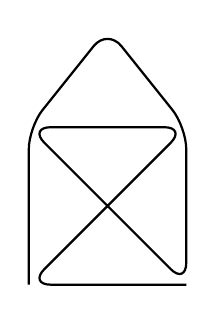
\begin{tikzpicture}
        \draw[thick, rounded corners=8pt]
                (0, 0) -- (0, 2) -- (1, 3.25) -- (2, 2) -- (2, 0) -- (0, 2) --
                (2, 2) -- (0, 0) -- (2, 0);
\end{tikzpicture}


\section{A Picture for Karl's Students}

\begin{figure}
\centering
        \tikz \draw (-1.5, 0) -- (1.5, 0) -- (0, -1.5) -- (0, 1.5);
\caption{Straight path construction}
\end{figure}

\begin{figure}
\centering
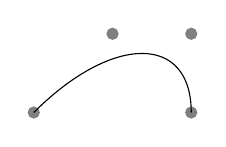
\begin{tikzpicture}
        \filldraw [gray] (0, 0) circle [radius=2pt]
                         (1, 1) circle [radius=2pt]
                         (2, 1) circle [radius=2pt]
                         (2, 0) circle [radius=2pt];
        \draw (0, 0) .. controls (1, 1) and (2, 1) .. (2, 0);
\end{tikzpicture}
\caption{Curved path construction}
\end{figure}

\vspace{1cm}

\begin{figure}
\centering
\begin{tikzpicture}
        \draw (-1.5, 0) -- (1.5, 0);
        \draw (0, -1.5) -- (0, 1.5);
        \draw (-1, 0) .. controls (-1, 0.555) and (-0.555, 1) .. (0, 1)
                .. controls (0.555, 1) and (1, 0.555) .. (1, 0);
\end{tikzpicture}
\caption{Half-circle with Bezier curves.}
\end{figure}

\vspace{1cm}

\tikz \draw[rotate=30] (0, 0) ellipse [x radius=20pt, y radius=10pt];

\vspace{1cm}

\begin{tikzpicture}
        \draw (-1.5, 0) -- (1.5, 0);
        \draw (0, -1.5) -- (0, 1.5);
        \draw (0, 0) circle [radius=1cm];
\end{tikzpicture}

\vspace{1cm}

\begin{figure}
\centering
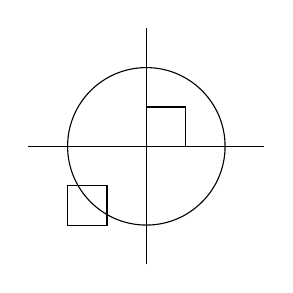
\begin{tikzpicture}
        \draw (-1.5, 0) -- (1.5, 0);
        \draw (0, -1.5) -- (0, 1.5);
        \draw (0, 0) circle [radius=1cm];
        \draw (0, 0) rectangle (0.5, 0.5);
        \draw (-0.5, -0.5) rectangle (-1, -1);
\end{tikzpicture}
\caption{Rectangle path construction.}
\end{figure}

\begin{figure}
\centering
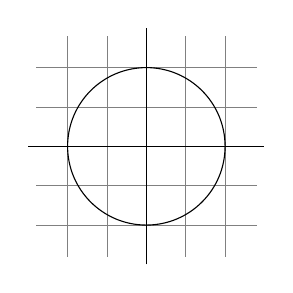
\begin{tikzpicture}
        \draw[step=.5cm, style=help lines] (-1.4, -1.4) grid (1.4, 1.4);
        \draw (-1.5, 0) -- (1.5, 0);
        \draw (0, -1.5) -- (0, 1.5);
        \draw (0, 0) circle [radius=1cm];
\end{tikzpicture}
\caption{Grid path construction.}
\end{figure}

\begin{figure}
\centering
\begin{tikzpicture}
        [Karl's grid/.style={help lines, color=#1!50},
         Karl's grid/.default=blue]

        \draw[Karl's grid] (0, 0) grid (1.5, 2);
        \draw[Karl's grid=red] (2, 0) grid (3.5, 2);
\end{tikzpicture}
\caption{Style setting.}
\end{figure}

\begin{figure}
\centering
\begin{tikzpicture}[scale=3]
        \draw (-1.5, 0) -- (1.5, 0);
        \draw (0, -1.5) -- (0, 1.5);
        \draw (0, 0) circle [radius=1cm];
        \draw (3mm, 0mm) arc [start angle=0, end angle=30, radius=3mm];
\end{tikzpicture}
\caption{Arc path construction.}
\end{figure}

\vspace{1cm}

\tikz \draw (0, 0) arc [start angle=0, end angle=315, x radius=1.75cm, y radius=1cm];

\vspace{1cm}

\begin{figure}
\centering
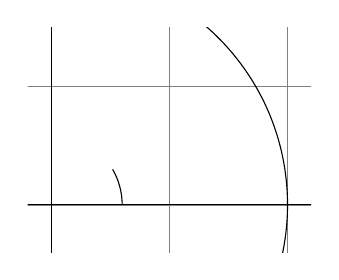
\begin{tikzpicture}[scale=3]
        \clip (-0.1, -0.2) rectangle (1.1, 0.75);
        \draw[step=.5cm, style=help lines] (-1.4, -1.4) grid (1.4, 1.4);
        \draw (-1.5, 0) -- (1.5, 0);
        \draw (0, -1.5) -- (0, 1.5);
        \draw (0, 0) circle [radius=1cm];
        \draw (3mm, 0mm) arc [start angle=0, end angle=30, radius=3mm];
\end{tikzpicture}
\caption{Clipping a path.}
\end{figure}

\begin{figure}
\centering
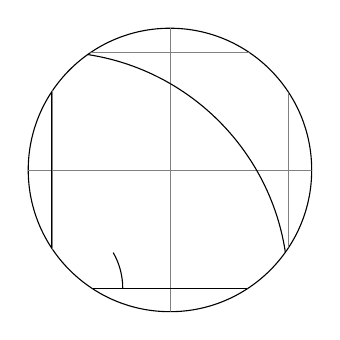
\begin{tikzpicture}[scale=3]
        \clip[draw] (0.5, 0.5) circle (.6cm);
        \draw[step=.5cm, style=help lines] (-1.4, -1.4) grid (1.4, 1.4);
        \draw (-1.5, 0) -- (1.5, 0);
        \draw (0, -1.5) -- (0, 1.5);
        \draw (0, 0) circle [radius=1cm];
        \draw (3mm, 0mm) arc [start angle=0, end angle=30, radius=3mm];
\end{tikzpicture}
\caption{Draw and clip a path.}
\end{figure}

\vspace{1cm}

\tikz \draw (0, 0) rectangle (1, 1) (0, 0) parabola (1, 1);

\vspace{1cm}

\tikz \draw[x=1pt, y=1pt] (0, 0) parabola bend (4, 16) (6, 12);

\vspace{1cm}

\begin{figure}
\centering
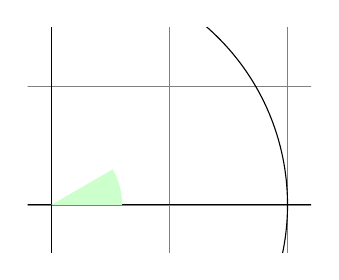
\begin{tikzpicture}[scale=3]
        \clip (-0.1, -0.2) rectangle (1.1, 0.75);
        \draw[step=.5cm, style=help lines] (-1.4, -1.4) grid (1.4, 1.4);
        \draw (-1.5, 0) -- (1.5, 0);
        \draw (0, -1.5) -- (0, 1.5);
        \draw (0, 0) circle [radius=1cm];
        \fill[green!20!white] (0, 0) -- (3mm, 0mm)
                arc [start angle=0, end angle=30, radius=3mm] -- cycle;
\end{tikzpicture}
\caption{Filling and drawing.}
\end{figure}

\begin{figure}
\centering
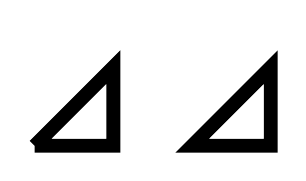
\begin{tikzpicture}[line width=5pt]
        \draw (0, 0) -- (1, 0) -- (1, 1) -- (0, 0);
        \draw (2, 0) -- (3, 0) -- (3, 1) -- cycle;
        \useasboundingbox (0, 1.5);  % make bounding box higher
\end{tikzpicture}
\caption{Triangles with cycle.}
\end{figure}

\begin{figure}
\centering
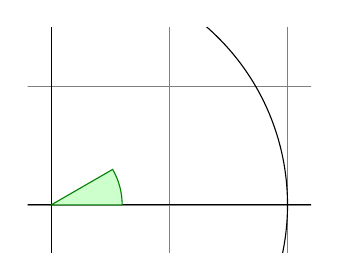
\begin{tikzpicture}[scale=3]
        \clip (-0.1, -0.2) rectangle (1.1, 0.75);
        \draw[step=.5cm, style=help lines] (-1.4, -1.4) grid (1.4, 1.4);
        \draw (-1.5, 0) -- (1.5, 0);
        \draw (0, -1.5) -- (0, 1.5);
        \draw (0, 0) circle [radius=1cm];
        \filldraw[fill=green!20!white, draw=green!50!black] (0, 0) -- (3mm, 0mm)
                arc [start angle=0, end angle=30, radius=3mm] -- cycle;
\end{tikzpicture}
\caption{Filling and drawing using filldraw.}
\end{figure}

\vspace{1cm}

\tikz \shade (0, 0) rectangle (2, 1) (3, 0.5) circle (.5cm);

\begin{figure}
\centering

\begin{tikzpicture}[rounded corners, ultra thick]
        \shade[top color=yellow, bottom color=black] (0, 0) rectangle +(2, 1);
\end{tikzpicture}
\caption{Coloured shading.}
\end{figure}

\begin{figure}
\centering
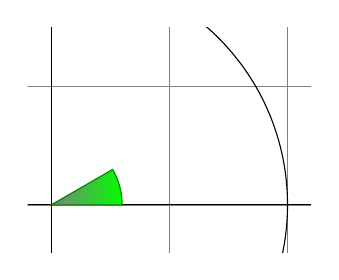
\begin{tikzpicture}[scale=3]
        \clip (-0.1, -0.2) rectangle (1.1, 0.75);
        \draw[step=.5cm, style=help lines] (-1.4, -1.4) grid (1.4, 1.4);
        \draw (-1.5, 0) -- (1.5, 0);
        \draw (0, -1.5) -- (0, 1.5);
        \draw (0, 0) circle [radius=1cm];
        \shadedraw[left color=gray, right color=green, draw=green!50!black]
                (0, 0) -- (3mm, 0mm)
                arc [start angle=0, end angle=30, radius=3mm] -- cycle;
\end{tikzpicture}
\caption{Filling and drawing using shadedraw.}
\end{figure}

\begin{figure}
\centering
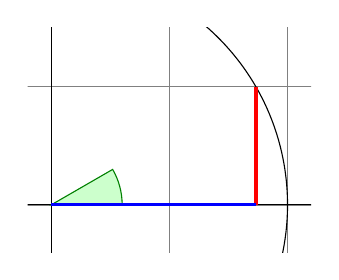
\begin{tikzpicture}[scale=3]
        \clip (-0.1, -0.2) rectangle (1.1, 0.75);
        \draw[step=.5cm, style=help lines] (-1.4, -1.4) grid (1.4, 1.4);
        \draw (-1.5, 0) -- (1.5, 0);
        \draw (0, -1.5) -- (0, 1.5);
        \draw (0, 0) circle [radius=1cm];
        \filldraw[fill=green!20!white, draw=green!50!black] (0, 0) -- (3mm, 0mm)
                arc [start angle=0, end angle=30, radius=3mm] -- cycle;
        \draw[red, very thick] (30:1cm) -- +(0, -0.5);
        \draw[blue, very thick] (30:1cm) ++(0, -0.5) -- (0, 0);
\end{tikzpicture}
\caption{Drawing lines using radial coordinates.}
\end{figure}

\begin{figure}
\centering
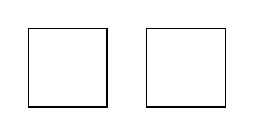
\begin{tikzpicture}
        \def\rectanglepath{-- ++(1cm, 0cm) -- ++(0cm, 1cm) -- ++(-1cm, 0cm) -- cycle}
        \draw (0, 0) \rectanglepath;
        \draw (1.5, 0) \rectanglepath;
\end{tikzpicture}
\caption{Rectangle path using ++, as opposed to using +.}
\end{figure}

\begin{figure}
\centering
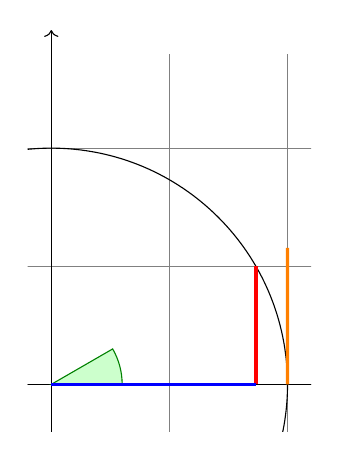
\begin{tikzpicture}[scale=3]
        \clip (-0.1, -0.2) rectangle (1.1, 1.51);
        \draw[step=.5cm, style=help lines] (-1.4, -1.4) grid (1.4, 1.4);
        \draw[->] (-1.5, 0) -- (1.5, 0);
        \draw[->] (0, -1.5) -- (0, 1.5);
        \draw (0, 0) circle [radius=1cm];
        \filldraw[fill=green!20!white, draw=green!50!black] (0, 0) -- (3mm, 0mm)
                arc [start angle=0, end angle=30, radius=3mm] -- cycle;
        \draw[red, very thick] (30:1cm) -- +(0, -0.5);
        \draw[blue, very thick] (30:1cm) ++(0, -0.5) -- (0, 0);

        \path [name path=upward line] (1, 0) -- (1, 1);
        \path [name path=sloped line] (0, 0) -- (30:1.5cm);

        \draw [name intersections={of=upward line and sloped line, by=x}]
              [very thick, orange] (1, 0) -- (x);
\end{tikzpicture}
\caption{Adding arrow tips.}
\end{figure}

\begin{figure}
\centering
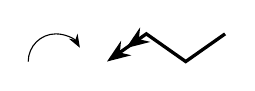
\begin{tikzpicture}[>=Stealth]
        \draw [->] (0, 0) arc [start angle=180, end angle=30, radius=10pt];
        \draw [<<-, very thick] (1, 0) -- (1.5cm, 10pt) -- (2cm, 0pt) -- (2.5cm, 10pt);
\end{tikzpicture}
\caption{Different kinds of arrow tips.}
\end{figure}

\begin{figure}
\centering
\begin{tikzpicture}[ultra thick]
        \draw (0, 0) -- (0, 1);
        \begin{scope}[thin]
                % NOTE(brendan): A useful tip: clipping using \clip is local to
                % a scope.
                \draw (1, 0) -- (1, 1);
                \draw (2, 0) -- (2, 1);
        \end{scope}
        \draw (3, 0) -- (3, 1);
\end{tikzpicture}
\caption{Scoping.}
\end{figure}

\vspace{1cm}

\tikz \draw (0, 0) -- (0, 0.5) [xshift=2pt] (0, 0) -- (0, 0.5);

\vspace{1cm}

\begin{figure}
\centering
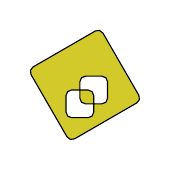
\begin{tikzpicture}[even odd rule, rounded corners=2pt, x=10pt, y=10pt]
        \filldraw[fill=yellow!80!black] (0, 0) rectangle (1, 1)
                [xshift=5pt, yshift=5pt] (0, 0) rectangle (1, 1)
                [rotate=30] (-1, -1) rectangle (2, 2);
\end{tikzpicture}
\caption{Change transformations in the middle of a path.}
\end{figure}

\vspace{1cm}

\foreach \x in {1, 2, 3} {$x = \x$, }

\begin{figure}
\centering
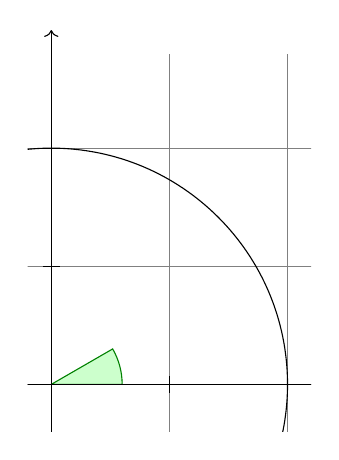
\begin{tikzpicture}[scale=3]
        \clip (-0.1, -0.2) rectangle (1.1, 1.51);
        \draw[step=.5cm, style=help lines] (-1.4, -1.4) grid (1.4, 1.4);
        \filldraw[fill=green!20!white, draw=green!50!black] (0, 0) -- (3mm, 0mm)
                arc [start angle=0, end angle=30, radius=3mm] -- cycle;
        \draw[->] (-1.5, 0) -- (1.5, 0);
        \draw[->] (0, -1.5) -- (0, 1.5);
        \draw (0, 0) circle [radius=1cm];

        \foreach \x in {0cm, 0.5cm, 1cm} \draw (\x, -1pt) -- (\x, 1pt);
        \foreach \y in {0cm, 0.5cm, 1cm} \draw (-1pt, \y) -- (1pt, \y);
\end{tikzpicture}
\caption{Adding ticks to axes using foreach.}
\end{figure}

\vspace{1cm}

\tikz \foreach \x in {1, ..., 10} \draw (\x, 0) circle (0.4cm);

\vspace{1cm}

\begin{figure}
\centering
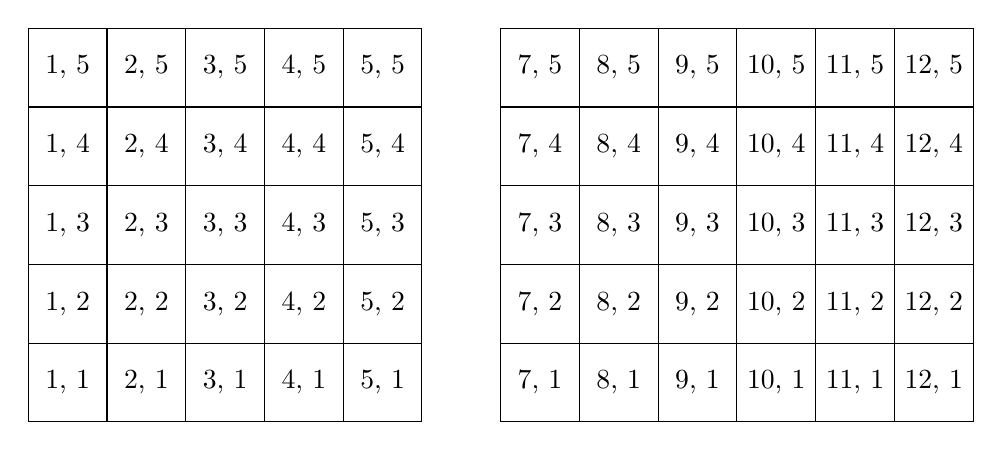
\begin{tikzpicture}
        \foreach \x in {1, 2, ..., 5, 7, 8, ..., 12}
        \foreach \y in {1, ..., 5}
        {
                \draw (\x, \y) +(-.5, -.5) rectangle ++(.5, .5);
                \draw (\x, \y) node{\x, \y};
        }
\end{tikzpicture}
\caption{Interesting effects with TikZ foreach.}
\end{figure}

\begin{figure}
\centering
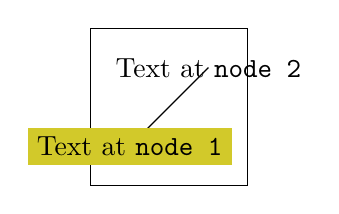
\begin{tikzpicture}
        \draw (0, 0) rectangle (2, 2);
        \draw (0.5, 0.5) node [fill=yellow!80!black]{Text at \verb!node 1!}
                -- (1.5, 1.5) node {Text at \verb!node 2!};
\end{tikzpicture}
\caption{Adding text.}
\end{figure}

\begin{figure}
\centering
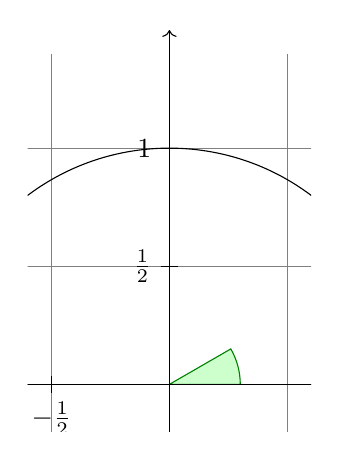
\begin{tikzpicture}[scale=3]
        \clip (-0.6, -0.2) rectangle (0.6, 1.51);
        \draw[step=.5cm, style=help lines] (-1.4, -1.4) grid (1.4, 1.4);
        \filldraw[fill=green!20!white, draw=green!50!black] (0, 0) -- (3mm, 0mm)
                arc [start angle=0, end angle=30, radius=3mm] -- cycle;
        \draw[->] (-1.5, 0) -- (1.5, 0);
        \draw[->] (0, -1.5) -- (0, 1.5);
        \draw (0, 0) circle [radius=1cm];

        \foreach \x/\xtext in {-1, -0.5/-\frac{1}{2}, 1}
                \draw (\x cm, 1pt) -- (\x cm, -1pt) node [anchor=north] {$\xtext$};
        \foreach \y/\ytext in {-1, -0.5/-\frac{1}{2}, 0.5/\frac{1}{2}, 1}
                \draw (1pt, \y cm) -- (-1pt, \y cm) node [anchor=east] {$\ytext$};
\end{tikzpicture}
\caption{Adding axes tick labels.}
\end{figure}

\begin{figure}
\centering
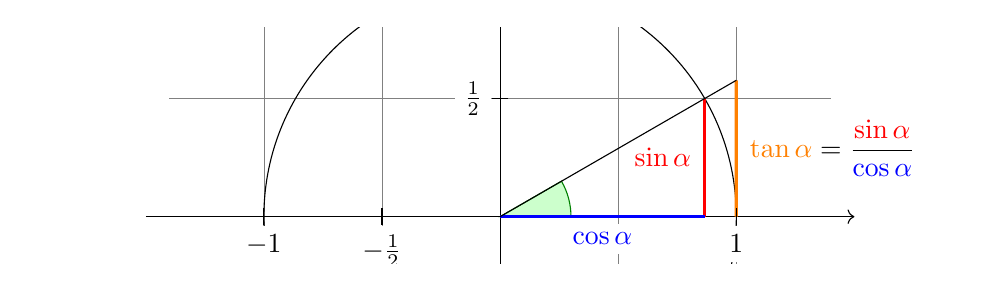
\begin{tikzpicture}[scale=3]
        \clip (-2, -0.2) rectangle (2, 0.8);
        \draw[step=.5cm, style=help lines] (-1.4, -1.4) grid (1.4, 1.4);
        \filldraw[fill=green!20!white, draw=green!50!black] (0, 0) -- (3mm, 0mm)
                arc [start angle=0, end angle=30, radius=3mm] -- cycle;
        \draw[->] (-1.5, 0) -- (1.5, 0) coordinate (x axis);
        \draw[->] (0, -1.5) -- (0, 1.5) coordinate (y axis);
        \draw (0, 0) circle [radius=1cm];

        \draw[red, very thick]
                (30:1cm) -- node [left=1pt, fill=white] {$\sin \alpha$} (30:1cm |- x axis);
        \draw[blue, very thick]
                (30:1cm |- x axis) -- node [below=2pt, fill=white] {$\cos \alpha$} (0, 0);

        \path [name path=upward line] (1, 0) -- (1, 1);
        \path [name path=sloped line] (0, 0) -- (30:1.5cm);
        \draw [name intersections={of=upward line and sloped line, by=t}]
              [very thick, orange] (1, 0) -- node [right=1pt, fill=white]
              {$\displaystyle \tan \alpha \color{black}=
                \frac{{\color{red}\sin \alpha}}{\color{blue}\cos \alpha}$} (t);

        \draw (0, 0) -- (t);

        \foreach \x/\xtext in {-1, -0.5/-\frac{1}{2}, 1}
                \draw (\x cm, 1pt) -- (\x cm, -1pt) node [anchor=north, fill=white] {$\xtext$};
        \foreach \y/\ytext in {-1, -0.5/-\frac{1}{2}, 0.5/\frac{1}{2}, 1}
                \draw (1pt, \y cm) -- (-1pt, \y cm) node [anchor=east, fill=white] {$\ytext$};
\end{tikzpicture}
\caption{Adding white fill to text.}
\end{figure}

\begin{figure}
\centering
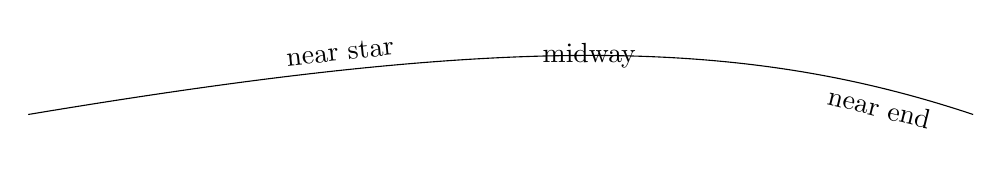
\begin{tikzpicture}
        \draw (0, 0) .. controls (6, 1) and (9, 1) ..
        node [near start, sloped, above] {near star}
        node {midway}
        node [very near end, sloped, below] {near end} (12, 0);
\end{tikzpicture}
\caption{Position labels on curves.}
\end{figure}

\begin{figure}
\centering
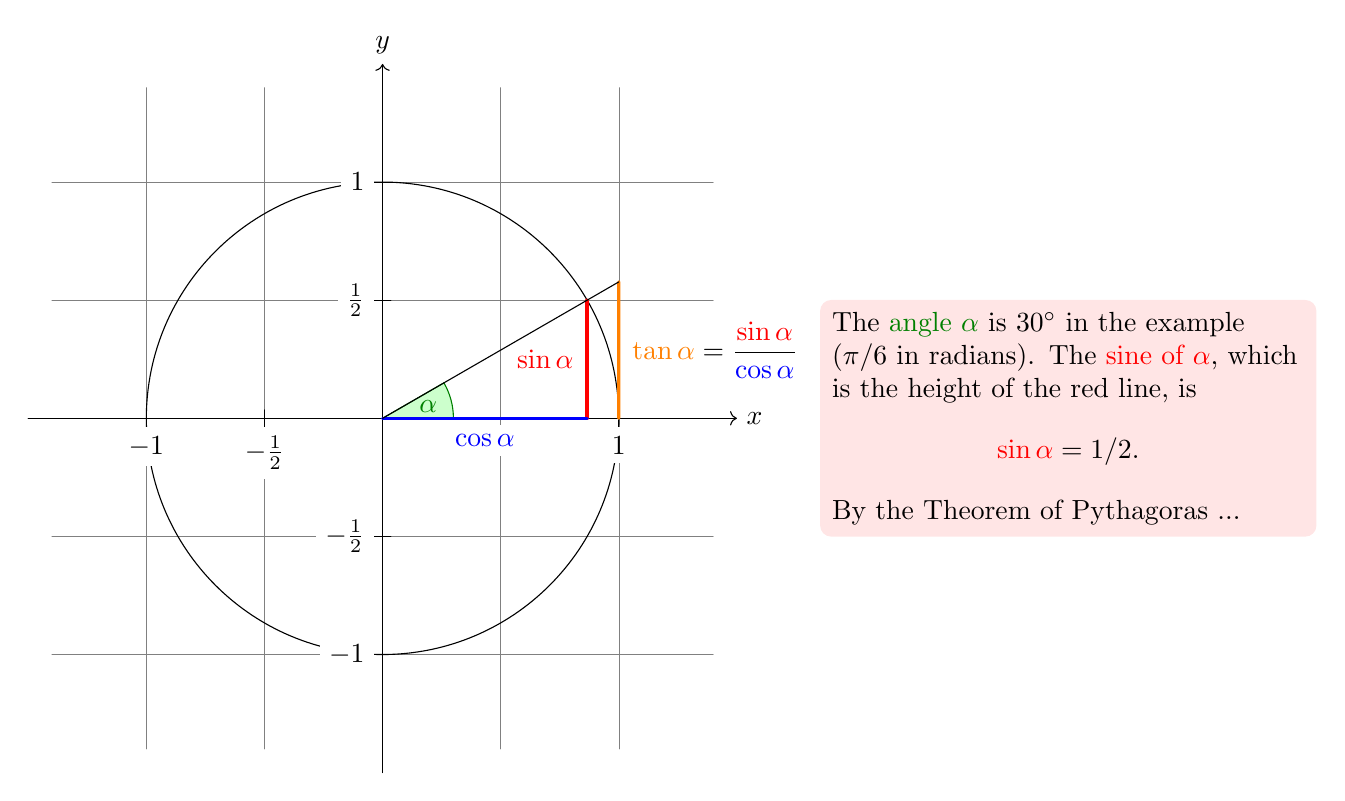
\begin{tikzpicture}
        [scale=3, line cap=round,
        % Styles
        axes/.style=,
        important line/.style={very thick},
        information text/.style={rounded corners, fill=red!10, inner sep=1ex}]

        % Colors
        \colorlet{anglecolor}{green!50!black}
        \colorlet{sincolor}{red}
        \colorlet{tancolor}{orange!80!black}
        \colorlet{coscolor}{blue}

        % The graphic
        \draw[step=.5cm, style=help lines] (-1.4, -1.4) grid (1.4, 1.4);

        \begin{scope}[axes]
                \draw[->] (-1.5, 0) -- (1.5, 0) node [right] {$x$} coordinate (x axis);
                \draw[->] (0, -1.5) -- (0, 1.5) node [above] {$y$} coordinate (y axis);
                \draw (0, 0) circle [radius=1cm];

                \foreach \x/\xtext in {-1, -0.5/-\frac{1}{2}, 1}
                \draw[xshift=\x cm] (0pt, 1pt) -- (0pt, -1pt) node [below, fill=white] {$\xtext$};
                \foreach \y/\ytext in {-1, -0.5/-\frac{1}{2}, 0.5/\frac{1}{2}, 1}
                \draw[yshift=\y cm] (1pt, 0pt) -- (-1pt, 0pt) node [left, fill=white] {$\ytext$};
        \end{scope}

        \filldraw[fill=green!20!white, draw=green!50!black] (0, 0) -- (3mm, 0mm)
                arc [start angle=0, end angle=30, radius=3mm] -- cycle;
        \draw (15:2mm) node [anglecolor] {$\alpha$};

        \draw[important line, sincolor]
                (30:1cm) -- node [left=1pt, fill=white] {$\sin \alpha$} (30:1cm |- x axis);
        \draw[important line, coscolor]
                (30:1cm |- x axis) -- node [below=2pt, fill=white] {$\cos \alpha$} (0, 0);

        \path [name path=upward line] (1, 0) -- (1, 1);
        \path [name path=sloped line] (0, 0) -- (30:1.5cm);
        \draw [name intersections={of=upward line and sloped line, by=t}]
              [very thick, orange] (1, 0) -- node [right=1pt, fill=white]
              {$\displaystyle \tan \alpha \color{black}=
                \frac{{\color{red}\sin \alpha}}{\color{blue}\cos \alpha}$} (t);

        \draw (0, 0) -- (t);

        \draw[xshift=1.85cm]
                node[right, text width=6cm, information text]
                {
                        The {\color{anglecolor} angle $\alpha$} is $30^\circ$ in the
                        example ($\pi/6$ in radians). The {\color{sincolor}sine of
                        $\alpha$}, which is the height of the red line, is
                        \[
                        {\color{sincolor} \sin \alpha} = 1/2.
                        \]
                        By the Theorem of Pythagoras ...
                };
\end{tikzpicture}
\caption{Full code with text label.}
\end{figure}

\begin{figure}
\centering
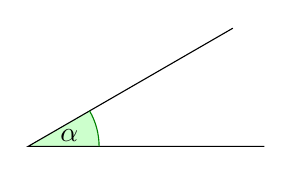
\begin{tikzpicture}[scale=3]
        \coordinate (A) at (1, 0);
        \coordinate (B) at (0, 0);
        \coordinate (C) at (30:1cm);

        \draw (A) -- (B) -- (C)
                pic
                [draw=green!50!black, fill=green!20, angle radius=9mm, "$\alpha$"]
                {angle=A--B--C};
\end{tikzpicture}
\caption{Using angle from pics.}
\end{figure}


\section{A Petri-Net for Hagen}

\newcommand{\circnode}[2]{\node at (#1, #2) [circle,draw] {}}
\newcommand{\rectnode}[2]{\node at (#1, #2) [rectangle,draw] {}}

\begin{figure}
\centering
\begin{tikzpicture}
        \circnode{0}{2};
        \circnode{0}{1};
        \circnode{0}{0};
        \rectnode{1}{1};
        \rectnode{-1}{1};
\end{tikzpicture}
\caption{Simple Petri net.}
\end{figure}

% NOTE(brendan): inner sep is the automatic space placed around text.
\tikzset{place/.style={circle,
                       draw=blue!50,
                       fill=blue!20,
                       thick,
                       inner sep=0pt,
                       minimum size=6mm},
         transition/.style={rectangle,
                            draw=black!50,
                            fill=black!20,
                            thick,
                            inner sep=0pt,
                            minimum size=4mm}}

\begin{figure}
\centering
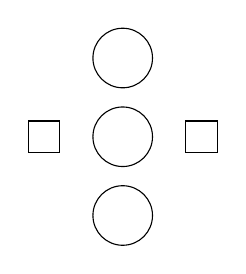
\begin{tikzpicture}
        \node[place] (waiting 1) at (0, 2) {};
        \node[place] (critical 1) at (0, 1) {};
        \node[transition] (semaphore) at (1, 1) {};
        \node[transition] (leave critical) at (-1, 1) {};
        \node[place] (enter critical) at (0, 0) {};
\end{tikzpicture}
\caption{Using styles.}
\end{figure}

\begin{figure}
\centering
\begin{tikzpicture}
        \node[place] (waiting) {};
        \node[place] (critical) [below=of waiting] {};
        \node[place] (semaphore) [below=of critical] {};
        \node[transition] (leave critical) [right=of critical] {};
        \node[transition] (enter critical) [left=of critical] {};

        \node[red, above] at (semaphore.north) {$s \leq 3$};
\end{tikzpicture}
\caption{Placing nodes using relative placement, and adding labels next to
         nodes.}
\end{figure}

\begin{figure}
\centering
\begin{tikzpicture}[every label/.style={red}]
        \node[place] (waiting) {};
        \node[place] (critical) [below=of waiting] {};
        \node[place] (semaphore) [below=of critical, label=above:$s \le 3$] {};
        \node[transition] (leave critical) [right=of critical] {};
        \node[transition] (enter critical) [left=of critical] {};
\end{tikzpicture}
\caption{Label.}
\end{figure}

\vspace{1cm}

\tikz \node [circle, draw, label=60:$60^\circ$, label=below:$-90^\circ$] {my circle};

\begin{figure}
\centering
\begin{tikzpicture}
        \node[place] (waiting) {};
        \node[place] (critical) [below=of waiting] {};
        \node[place] (semaphore) [below=of critical] {};
        \node[transition] (leave critical) [right=of critical] {};
        \node[transition] (enter critical) [left=of critical] {};

        \draw [->] (enter critical) -- (critical);
        \draw [->] (waiting) .. controls +(left:8mm) and +(up:8mm)
                .. (enter critical);
\end{tikzpicture}
\caption{Connecting nodes.}
\end{figure}

\begin{figure}
\centering
\begin{tikzpicture}
        \node[place] (waiting) {};
        \node[place] (critical) [below=of waiting] {};
        \node[place] (semaphore) [below=of critical] {};
        \node[transition] (leave critical) [right=of critical] {};
        \node[transition] (enter critical) [left=of critical] {};

        \draw [->] (enter critical) to (critical);
        \draw [->] (waiting) to [out=180, in=90] (enter critical);
\end{tikzpicture}
\caption{Using angles to control connection lines.}
\end{figure}

\begin{figure}
\centering
\begin{tikzpicture}
        \node[place] (waiting) {};
        \node[place] (critical) [below=of waiting] {};
        \node[place] (semaphore) [below=of critical] {};
        \node[transition] (leave critical) [right=of critical] {};
        \node[transition] (enter critical) [left=of critical] {};

        \draw [->] (enter critical) to (critical);
        \draw [->] (waiting) to [bend right=45] (enter critical);
        \draw [->] (enter critical) to [bend right=45] (semaphore);
\end{tikzpicture}
\caption{Control angles using bends.}
\end{figure}

\begin{figure}
\centering
\begin{tikzpicture}
        \node[place] (waiting) {};
        \node[place] (critical) [below=of waiting] {};
        \node[place] (semaphore) [below=of critical] {};
        \node[transition] (leave critical) [right=of critical] {};
        \node[transition] (enter critical) [left=of critical] {}
                edge [->] (critical)
                edge [<-, bend left=45] (waiting)
                edge [->, bend right=45] (semaphore);
\end{tikzpicture}
\caption{Edges.}
\end{figure}

\begin{figure}
\centering
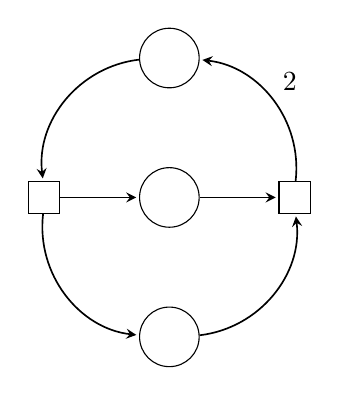
\begin{tikzpicture}
        [bend angle=45,
         pre/.style={<-, shorten <= 1pt, >=stealth, semithick},
         post/.style={->, shorten >= 1pt, >=stealth, semithick}]

        \node[place] (waiting) {};
        \node[place] (critical) [below=of waiting] {};
        \node[place] (semaphore) [below=of critical] {};

        \node[transition] (leave critical) [right=of critical] {}
                edge [pre] (critical)
                edge [post, bend right] node [auto, swap] {2} (waiting)
                edge [pre, bend left] (semaphore);
        \node[transition] (enter critical) [left=of critical] {}
                edge [post] (critical)
                edge [pre, bend left] (waiting)
                edge [post, bend right] (semaphore);
\end{tikzpicture}
\caption{Using pre and post.}
\end{figure}

\vspace{1cm}

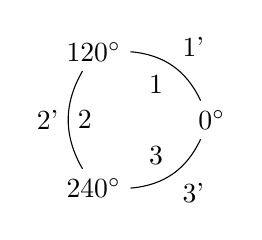
\begin{tikzpicture}[auto, bend right]
        \node (a) at (0:1) {$0^\circ$};
        \node (b) at (120:1) {$120^\circ$};
        \node (c) at (240:1) {$240^\circ$};

        \draw (a) to node {1} node [swap] {1'} (b)
                (b) to node {2} node [swap] {2'} (c)
                (c) to node {3} node [swap] {3'} (a);
\end{tikzpicture}

\vspace{1cm}

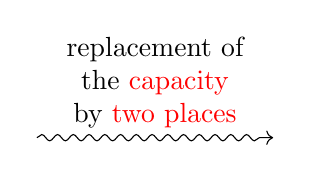
\begin{tikzpicture}
        \draw [->, decorate, decoration={snake,
                                         amplitude=.4mm,
                                         segment length=2mm,
                                         post length=1mm}]
               (0, 0) -- (3, 0)
               node [above, align=center, midway, text width=3cm]
               {
                       replacement of the \textcolor{red}{capacity} by
                       \textcolor{red}{two places}
               };
\end{tikzpicture}

\vspace{1cm}

\tikzset{pre/.style={<-, shorten <= 1pt, >=stealth, semithick},
         post/.style={->, shorten >= 1pt, >=stealth, semithick}}

\begin{figure}
\centering
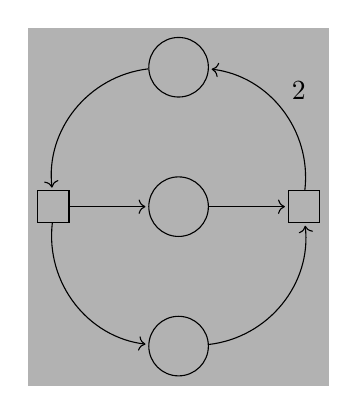
\begin{tikzpicture}[bend angle=45]
        \node[place] (waiting) {};
        \node[place] (critical) [below=of waiting] {};
        \node[place] (semaphore) [below=of critical] {};

        \node[transition] (leave critical) [right=of critical] {}
                edge [pre] (critical)
                edge [post, bend right] node [auto, swap] {2} (waiting)
                edge [pre, bend left] (semaphore);
        \node[transition] (enter critical) [left=of critical] {}
                edge [post] (critical)
                edge [pre, bend left] (waiting)
                edge [post, bend right] (semaphore);

        \begin{scope}[on background layer]
                \node [fill=black!30, fit=(waiting) (critical) (semaphore)
                        (enter critical) (leave critical)] {};
        \end{scope}
\end{tikzpicture}
\caption{Background layers.}
\end{figure}

\begin{figure}
\centering
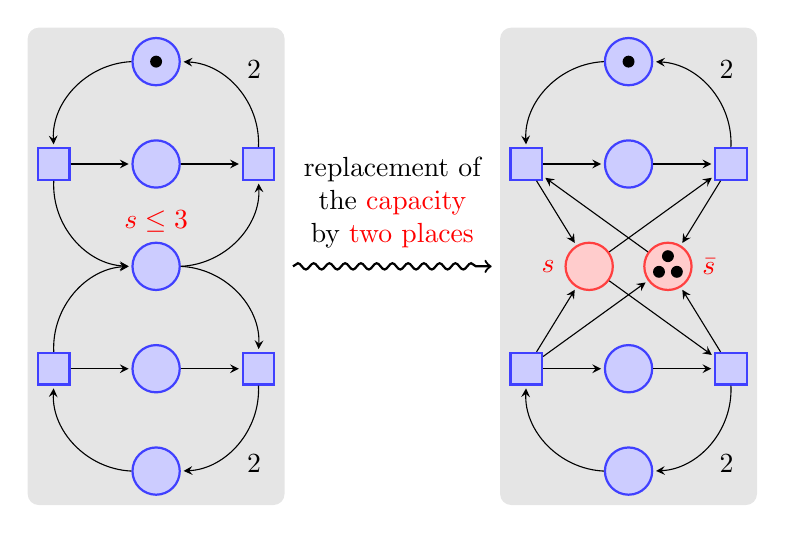
\begin{tikzpicture}
        [node distance=1.3cm,
        on grid,
        >=stealth,
        bend angle=45,
        auto,
        every place/.style={minimum size=6mm, thick, draw=blue!75, fill=blue!20},
        every transition/.style={thick, draw=blue!75, fill=blue!20},
        red place/.style={place, draw=red!75, fill=red!20},
        every label/.style={red}]

        \node[place, tokens=1] (w1) {};
        \node[place] (c1) [below=of w1] {};
        \node[place] (s) [below=of c1, label=above:$s \le 3$] {};
        \node[place] (c2) [below=of s] {};
        \node[place] (w2) [below=of c2] {};

        \node [transition] (e1) [left=of c1] {}
                edge [pre,bend left] (w1)
                edge [post,bend right] (s)
                edge [post] (c1);
        \node [transition] (e2) [left=of c2] {}
                edge [pre,bend right] (w2)
                edge [post,bend left] (s)
                edge [post] (c2);
        \node [transition] (l1) [right=of c1] {}
                edge [pre] (c1)
                edge [pre,bend left] (s)
                edge [post,bend right] node[swap] {2} (w1);
        \node [transition] (l2) [right=of c2] {}
                edge [pre] (c2)
                edge [pre,bend right] (s)
                edge [post,bend left] node {2} (w2);

        \begin{scope}[xshift=6cm]
                \node[place, tokens=1] (w1') {};
                \node[place] (c1') [below=of w1'] {};
                \node[red place] (s1') [below=of c1', xshift=-5mm] [label=left:$s$] {};
                \node[red place, tokens=3] (s2') [below=of c1', xshift=5mm] [label=right:$\bar{s}$] {};
                \node[place] (c2') [below=of s1', xshift=5mm] {};
                \node[place] (w2') [below=of c2'] {};

                \node [transition] (e1') [left=of c1'] {}
                        edge [pre,bend left] (w1')
                        edge [post] (s1')
                        edge [pre] (s2')
                        edge [post] (c1');
                \node [transition] (e2') [left=of c2'] {}
                        edge [pre,bend right] (w2')
                        edge [post] (s1')
                        edge [post] (s2')
                        edge [post] (c2');
                \node [transition] (l1') [right=of c1'] {}
                        edge [pre] (c1')
                        edge [pre] (s1')
                        edge [post] (s2')
                        edge [post,bend right] node[swap] {2} (w1');
                \node [transition] (l2') [right=of c2'] {}
                        edge [pre] (c2')
                        edge [pre] (s1')
                        edge [post] (s2')
                        edge [post,bend left] node {2} (w2');
        \end{scope}

        \begin{scope}[on background layer]
                \node (r1) [fill=black!10, rounded corners, fit=(w1)(w2)(e1)(e2)(l1)(l2)] {};
                \node (r2) [fill=black!10, rounded corners, fit=(w1')(w2')(e1')(e2')(l1')(l2')] {};
        \end{scope}

        \draw [shorten >=1mm,
               -to,
               thick,
               decorate,
               decoration={snake, amplitude=.4mm, segment length=2mm, pre=moveto, pre length=1mm, post length=2mm}]
               (r1) -- (r2)
               node [above=1mm, align=center, midway, text width=3cm]
               {
                       replacement of the \textcolor{red}{capacity} by
                       \textcolor{red}{two places}
               };
\end{tikzpicture}
\caption{The complete code.}
\end{figure}

\end{document}
